\documentclass[a3paper]{article}

\usepackage[left=5mm,right=5mm,top=8.5mm,bottom=8.5mm]{geometry}
\pagestyle{empty}
\usepackage{tikz}
\usetikzlibrary{
    decorations.markings,
    decorations.pathmorphing,
    decorations.text,
}
\usepackage{graphicx}
\usepackage{eucal}
\usepackage{contour}
\contourlength{0.05mm}
\usepackage{fontspec}
\newfontface\textlino{QTLinoscroll}
% \usepackage{yfonts}
% \usepackage{dozenal}

\newcommand{\insR}{8mm}
\newcommand{\midR}{20mm}
\newcommand{\outR}{67mm}
\newcommand{\E}{\reflectbox{3}}
\newcommand{\X}{$\mathcal{X}$}

\begin{document}
\begin{center}
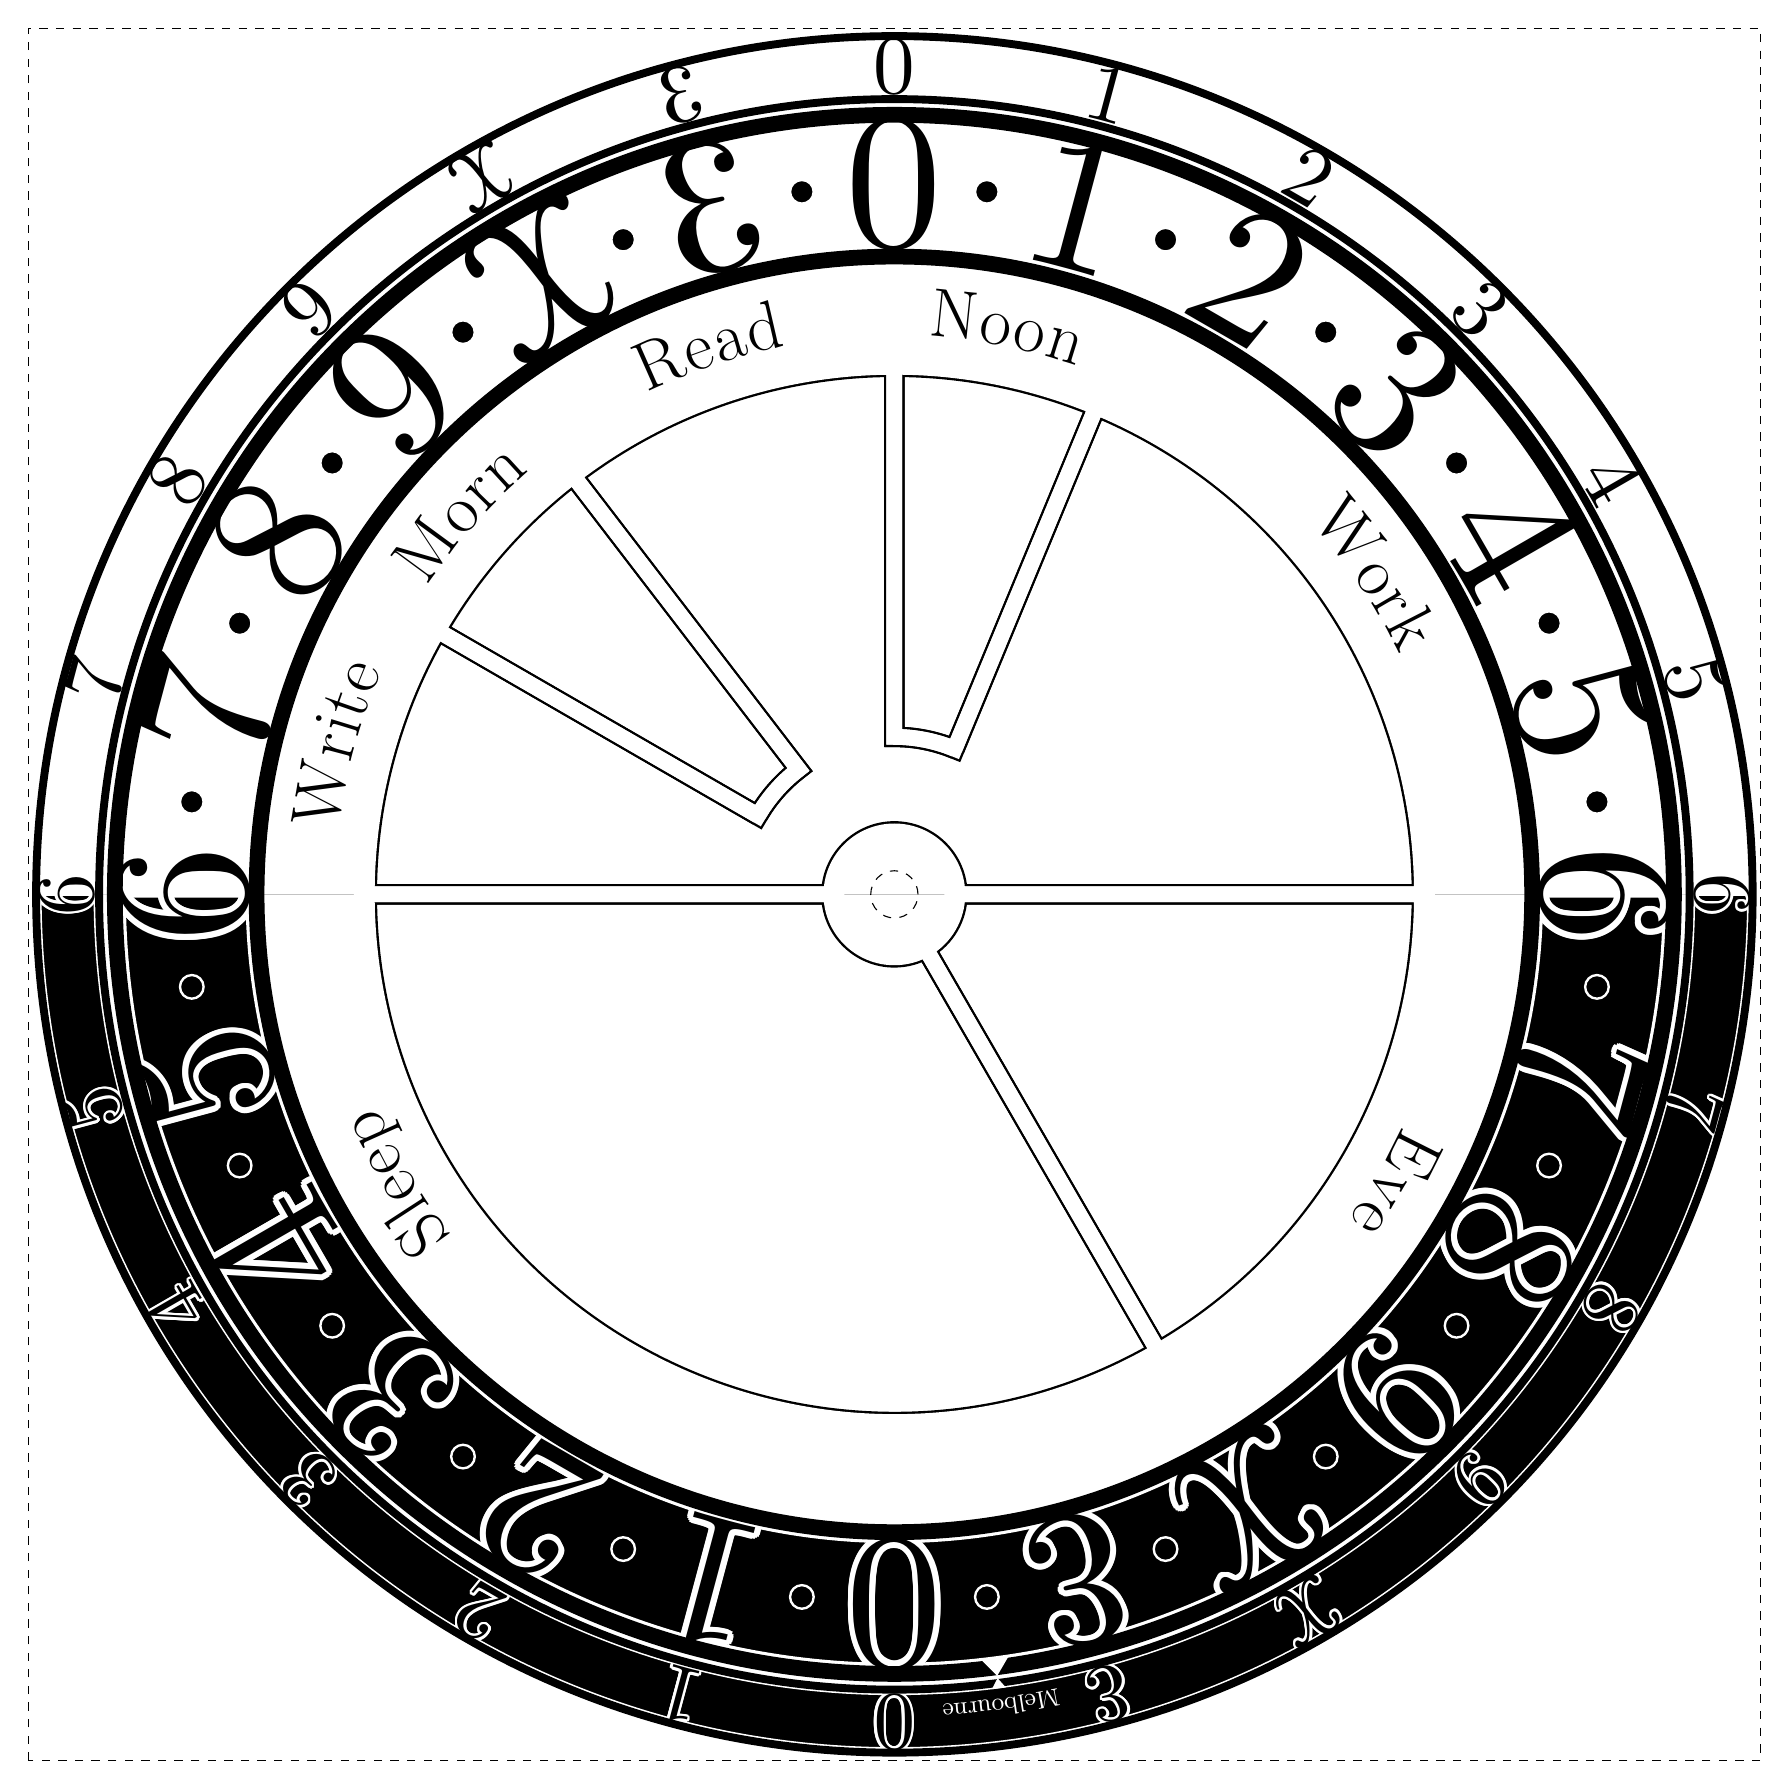
\begin{tikzpicture}
    % BORDER
    \draw[dashed] (-110mm,-110mm) rectangle (110mm,110mm);
    \draw[dashed] (0,0) circle [radius=3mm];

    % OUTER RING
    % Background
    \draw[fill=black,draw=white,line width=.4mm]
        (180:101.5mm) -- (180:108.5mm) arc (180:360:108.5mm)
        (360:108.5mm) -- (360:101.5mm) arc (360:180:101.5mm);
    % Numerals
    \foreach \angle/\label in {%
            270/0,255/1,240/2,225/3,210/4,195/5,%
            180/6,165/7,150/8,135/9,120/\X,105/\E%
    } {
        \node[rotate=\angle-90,scale=3,inner sep=0pt]
            at (\angle:105mm) {\contour{white}{\label}};
        \node[rotate=\angle+90,scale=3,inner sep=0pt]
            at (\angle-180:105mm) {\contour{white}{\label}};
    }
    % Borders
    \draw [line width=1mm] (0,0) circle [radius=110mm-1mm];
    \draw [line width=1mm] (0,0) circle [radius=100mm+1mm];
    \foreach \angle/\tz in {%
            270/Melbourne%
    } {
        \path[postaction={decorate,decoration={text align={center},%
            raise={-2mm},text along path,text={|\small\color{white}|\tz}}}]
            (\angle+15:105mm) arc (\angle+15:\angle:105mm);
        \path[fill=white]
            (\angle+7.5:100.4mm)--(\angle+7:101.7mm)--(\angle+8:101.7mm);
        
    }
    
    % NUMBERS
    % Background
    \draw[fill=black,draw=white,line width=.8mm]
        (180:82mm) -- (180:98mm) arc (180:360:98mm)
        (360:98mm) -- (360:82mm) arc (360:180:82mm);
    % Numerals
    \foreach \angle/\label in {%
            270/0,255/1,240/2,225/3,210/4,195/5,%
            180/6,165/7,150/8,135/9,120/\X,105/\E%
    } {
        \node[rotate=\angle-90,scale=7,inner sep=0pt]
            at (\angle:90mm-.15mm) {\contour{white}{\label}};
        \node[rotate=\angle+90,scale=7,inner sep=0pt]
            at (\angle-180:90mm-.15mm) {\contour{white}{\label}};
    }
    % Little Circles
    \foreach \angle in {-90,-75,...,255} { % 24ths
        \draw[fill,draw=white,line width=.3mm]
            (\angle+7.5:90mm) circle [radius=1.5mm];
    }
    % Borders
    \draw [line width=2mm] (0,0) circle [radius=100mm-1mm];
    \draw [line width=2mm] (0,0) circle [radius=80mm+1mm];

    % FACE
    % Sectors
    \foreach \lcolor/\lwidth in {black/2.6mm,white/2mm} {
    \begin{scope}[every path/.style={draw=\lcolor,line width=\lwidth}]
        \draw (180:\insR)   -- (180:\outR)   arc(180:150:\outR)     --
              (150:\outR)   -- (150:\midR)   arc(150:127.5:\midR)   --
              (127.5:\midR) -- (127.5:\outR) arc(127.5:90:\outR)    --
              (90:\outR)    -- (90:\midR)    arc(90:67.5:\midR)     --
              (67.5:\midR)  -- (67.5:\outR)  arc(67.5:0:\outR)      --
              (0:\outR)     -- (0:\insR)     arc(0:180:\insR)       ;
        \draw (0:\insR)     -- (0:\outR)     arc(0:-60:\outR)       --
              (-60:\outR)   -- (-60:\insR)   arc(-60:0:\insR)       ;
        \draw (300:\insR)   -- (300:\outR)   arc(300:180:\outR)     --
              (180:\outR)   -- (180:\insR)   arc(180:300:\insR)     ;
        \draw (150:\midR)   -- (150:\outR)   arc(150:127.5:\outR)   --
              (127.5:\outR) -- (127.5:\midR) arc(127.5:150:\midR)   ;
        \draw (67.5:\midR)  -- (67.5:\outR)  arc(67.5:90:\outR)     --
              (90:\outR)    -- (90:\midR)    arc(90:67.5:\midR)     ;
    \end{scope}
    }
    % (Cover up external lines)
    \draw[line width=1mm,draw=white] (0,0) circle (\outR+1.15mm);
    \draw[line width=1mm,draw=white] (0,0) circle (\insR-1.15mm);
    % Labels
    \foreach \phi/\label in {180/Write,153.75/Morn,123.75/Read,93.75/Noon,%
        48.75/Work,345/Eve,225/Sleep} {
        \path[postaction={decorate,decoration={text align={center},%
            raise={4mm},text along path,text={|\Huge\textlino|\label}}}]
            (\phi:\outR) arc (\phi:\phi-30:\outR);
        }
    % arc(0:-60:\outR) node[pos=0.25,sloped,above] {Evening}
    % arc(300:180:\outR) node[pos=0.875,sloped,above] {Sleeping}

    % POINTER
    \path[fill=white] (277.5:100.1mm) -- (276.5:97.9mm) -- (278.5:97.9mm);
    
\end{tikzpicture}
\end{center}
        
% VARIOUS TRANSDECIMALS
% \begin{center}
% \begin{tikzpicture}[every node/.style={scale=7}]
% \node at (-25mm,0) {23};
% \node[yscale=-1,xscale=-1] at (-6mm,0) {2};
% \node[xscale=-1] at (+6mm,0) {3};
% \node at (+25mm,0) {\x\e};
% % \node at (0,+25mm) {\textturnthree\textturntwo};
% \node at (0,-25mm) {$\mathcal{XE}$};
% \node at (+25mm,-25mm) {$\chi\mathcal{E}$};
% \end{tikzpicture}
% \end{center}

\end{document}
